% !TEX root = ./main.tex
% Resume

% !TEX root = ./main.tex

\documentclass{article}
\usepackage[a4paper, textwidth=180mm, textheight=260mm]{geometry}
\usepackage[hidelinks, colorlinks=true]{hyperref}
\usepackage{graphicx}
\usepackage{booktabs}
\usepackage{tikz}

% Configurations
\setlength{\parindent}{0pt}
\pagestyle{empty}

% Symbols
\newcommand{\symbolHt}{1.2em}
\newcommand{\phoneChar}{
    \begingroup\normalfont
    \raisebox{-0.08cm}{ % '%' for no space in end
        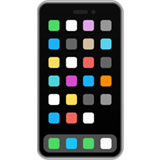
\includegraphics[height=\symbolHt]{icons/phone.png}}%
    \endgroup
}
\newcommand{\homeChar}{
    \begingroup\normalfont
    \raisebox{-0.05cm}{
        
\includegraphics[height=\symbolHt]{icons/house.png}}
    \endgroup
}
\newcommand{\githubChar}{
    \begingroup\normalfont
    % From: https://www.flaticon.com/free-icon/github_2111432?term=github&page=1&position=4&origin=search&related_id=2111432
    \raisebox{-0.07cm}{
        
\includegraphics[height=\symbolHt]{icons/github.png}}
    \endgroup
}
\newcommand{\webChar}{
    \begingroup\normalfont
    % From: https://www.flaticon.com/free-icon/world-wide-web_1006771?term=website&page=1&position=1&origin=search&related_id=1006771
    \raisebox{-0.07cm}{
        
\includegraphics[height=\symbolHt]{icons/world-wide-web.png}}
    \endgroup
}
\newcommand{\linkedinChar}{
    \begingroup\normalfont
    % From: https://www.flaticon.com/free-icon/linkedin_3536505?term=linkedin&page=1&position=1&origin=search&related_id=3536505
    \raisebox{-0.07cm}{
        
\includegraphics[height=\symbolHt]{icons/linkedin.png}}
    \endgroup
}
% New section
\newcommand{\newsec}[1]{
    {\bf \large #1}
    \vspace{2mm}
    \hrule
    \vspace{2mm}
}
% New education header [Degree, Institute, Date \n \hfill GPA]
\newcommand{\eduheader}[5]{
    \begin{minipage}{\linewidth}
        \vspace{1mm}
        {\bf #1} \hfill {\it #2} \hfill #3 \hfill \\
        \rightline{\bf #4}
        \vspace{-8mm}
        {#5}
        \vspace{1mm}
    \end{minipage}
}
% New experience header
\newcommand{\expheader}[4]{
    \begin{minipage}{\linewidth}
        \vspace{1mm}
        {\bf #1} \hfill {\it #2} \hfill #3
        {#4}
        \vspace{1mm}
    \end{minipage}
}

\begin{document}
    {
    \hfill
    \begin{minipage}{0.85\textwidth}
        \begin{center}
            {\bf \LARGE Avneesh Mishra} 
            \\ [4mm] \hfill                 % Phone number
            \phoneChar +91 99163 32393 
            \hfill                          % Email address
            \texttt{123avneesh@gmail.com} 
            \hfill                          % Address
            \homeChar Bengaluru, Karnataka, IN 
            \hfill { } \\ [1mm] \hfill      % Blog
            \webChar \href{https://theprojectsguy.github.io/}{
                theprojectsguy.github.io} 
            \hfill                          % Linkedin
            \linkedinChar \href{
                https://www.linkedin.com/in/avneesh-mishra/}{
                avneesh-mishra}
            \hfill                          % GitHub
            \githubChar \href{https://github.com/TheProjectsGuy}{
                TheProjectsGuy}
            \hfill { } \\
        \end{center}
    \end{minipage}
    \begin{minipage}{0.1\textwidth}
        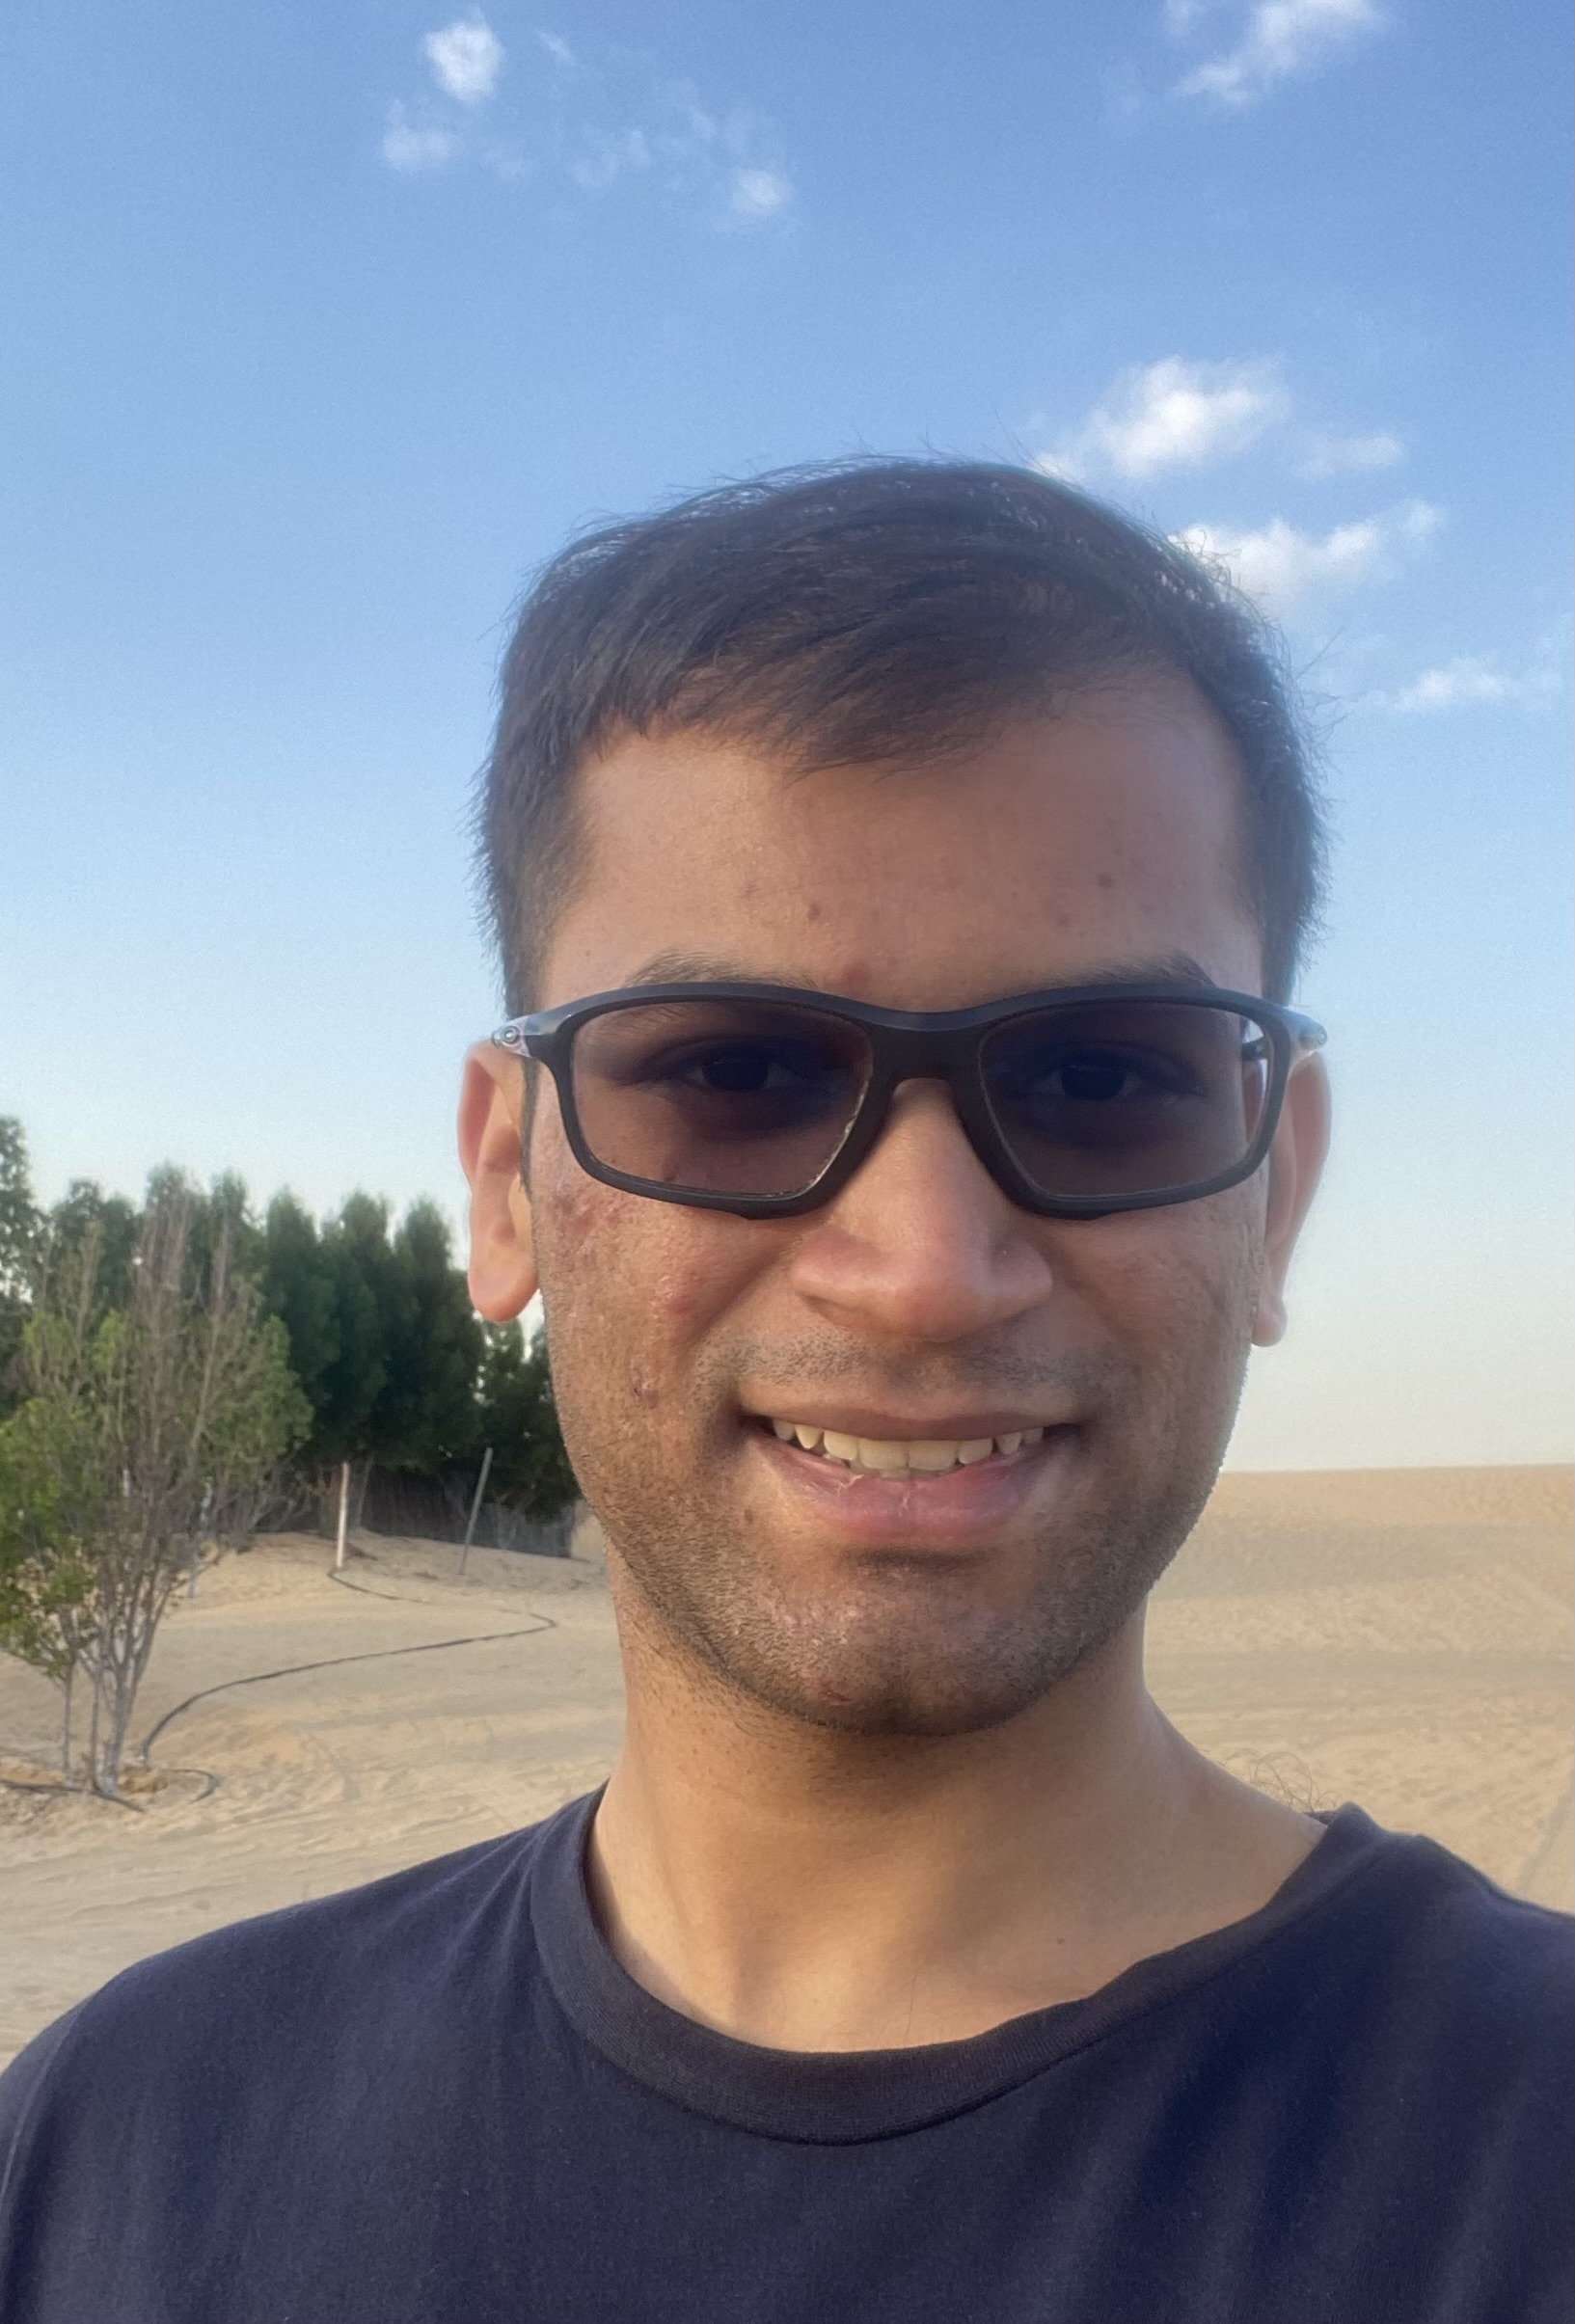
\includegraphics[width=\linewidth]{me.jpg}
    \end{minipage} \\
    }
    % --------------------- Main profile ---------------------
    \newsec{Profile}
    A Computer Vision and AI researcher from IIIT-H with a background in
    Robotics and Mechatronics engineering. Skilled at developing and
    deploying cutting-edge research from literature to hosting. Other
    skills include system administration and full-stack web development.
    \\ [4mm]
    % ----------------- Areas of experience -----------------
    \newsec{Areas of Experience}
    \begin{tabular}{cp{0.9\textwidth}}
        \raisebox{-0.8cm}{  % Strong
        \tikz \fill [green, draw=black] (0.0,0.0) rectangle (0.2, 1.0);
        } & % ------ Strong suits ------
        Computer Vision (SLAM systems, Image and video) - AI (PyTorch,
        TensorFlow, WandB) - Computer Science (Linux, MacOS, Windows;
        Docker; OS \& Hardware) - Programming (Python, Bash/Shell, C++) -
        Frameworks (Pandas, OpenCV, Open3D, ROS) 
        \\ [1mm]
        \raisebox{-1cm}{  % Medium
        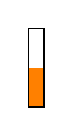
\begin{tikzpicture}
            \fill [orange] (0.0, 0.0) rectangle (0.2, 0.5);
            \draw [black]  (0.0, 0.0) rectangle (0.2, 1.0);
        \end{tikzpicture}
        } & % ------ Weak suits ------
        Systems Administration (HPC, IAM, NAS, FreeIPA, Networking,
        Storage, Hardware) - Cloud (AWS, Linode, Runpod) - Application
        Development (Python, Web, Unity AR) - CI/CD Pipelines - Programming
        (MATLAB, Javascript, C, Swift) - Embedded Systems (Jetson, ATmega,
        STM32, TI, FPGAs) - CAD (Electronics: KiCAD; Mechanical: Fusion
        360, SolidWorks) \\ [1mm] & {\bf Hobbies:} Reading, finance,
        cooking
    \end{tabular}
    \\ [4mm]
    % ------------------------ Education ------------------------
    \newsec{Education}
    \eduheader{M.S. by Research (CSE)}{
            \href{https://robotics.iiit.ac.in/}
                {Robotics Research Center} (RRC), 
                IIIT Hyderabad}{
            August 2021 to July 2024}{
            CGPA 10/10}{
    \begin{itemize}
        \setlength{\itemsep}{0mm}
        \item Thesis: \href{https://github.com/TheProjectsGuy/IIITH-MS-Thesis}{Foundation Models for Visual Place Recognition}
        \item RRC Summer School 2022 - Multi-View Geometry (\href{https://github.com/TheProjectsGuy/RRC22-Summer-School-MVG4}{GitHub})
        \item SLAM (Simultaneous Localization and Mapping) using cameras,
            VPR systems, local features matching, global image descriptors.
        \item Group equivariant deep learning, rotation robust descriptors
            for feature matching
        \item Courses: Computer Vision, Statistical Methods in AI, and
            Mobile Robotics
        \item Student SysAdmin (from May 2022 to Feb 2023)
    \end{itemize}
    }
    \eduheader{B.Tech. in Mechatronics Engineering}{
            \href{https://www.manipal.edu/mit.html}
                {Manipal Institute of Technology}}{
            July 2016 to July 2020}{CGPA 9.88/10 (Gold Medalist)}{
    \begin{itemize}
        \setlength{\itemsep}{0mm}
        \item Minor in Robotics and Artificial Intelligence
        \item Quarter-finalist for IICDC (DST\&TI) 2018
        \item Technical Head of ISA (Manipal Chapter)
        \item Research head of RoboManipal (Robotics student project) and
            organized RoboWars (event) for TechTatva. Participated in
            RoboCon 2018.
    \end{itemize}
    }
    % ----------------------- Experience -----------------------
    \newsec{Experience}
    \expheader{Consultant}{
        \href{https://www.hitloop.it/}{Hitloop}, Hyderabad}{
        July 2023 to November 2023}{
    \begin{itemize}
        \item Google Mediapipe and OpenMMLab solutions for detecting pose
            and facial landmarks.
        \item Dubbing use-cases for multi-lingual content creation.
            Lip-sync and voice cloning.
    \end{itemize}}
    \expheader{System Administrator}{RRC, IIIT Hyderabad}{
        May 2022 to Feb 2023}{
    \begin{itemize}
        \item Assisted in maintaining a SLURM HPC cluster with NFS, RAID,
            and networking components.
        \item Oversaw FreeIPA computing environment of RRC for simulation
            servers. Multi-user access and dataset storage. Developed 
            shell scripts for report generation, user management, and HPC
            job scheduling.
        \item Assembled powerful workstations with multiple GPUs. Ensured
            high up-time of servers through continuous Netdata monitoring
            and alerts.
        \item Created and maintained documentation and custom scripts for
            RRC simulation servers and Ada HPC system.
    \end{itemize}}
    \expheader{Consultant}{
        \href{https://artpark.in/}{Artpark}, RBCCPS, IISc Bangalore}{
        March 2021 to August 2021}{
    \begin{itemize}
        \setlength{\itemsep}{0mm}
        \item Teleoperation using Asha (\href{
            https://www.hansonrobotics.com/sophia/}{Sophia} from 
            Hanson Robotics) with Team Aham for the \href{
            https://avatar.xprize.org/prizes/avatar}{ANA Avatar 
            XPrize} challenge.
        \item Experience with HTC Vive (AR/VR) in Unity. Also worked
            with ROS (RViZ, kinematics) and Eigen.
        \item \href{https://www.youtube.com/watch?v=jTkIXtf35w8}{Teleoperation} of a KUKA robotic arm and
            \href{https://www.youtube.com/watch?v=_vVxpMM_nbQ}{web-streaming
            setup} to measure end-to-end latency (using USB/IP).
    \end{itemize}}
    \expheader{Student Intern}{
        \href{https://www.drdo.gov.in/drdo/labs-and-establishments/centre-artificial-intelligence-robotics-cair}{CAIR}, 
        DRDO, Bangalore}{December 2019 to July 2020}{
    \begin{itemize}
        \setlength{\itemsep}{0mm}
        \item Developed a quadruped test platform (software and
            embedded program) to execute gaits for my
            \href{https://www.dropbox.com/scl/fi/ntwybuhk6n4kn3bfkkesc/BTech-Mechatronics-Endterm-Report.pdf?rlkey=buo9s7dxvl8ohvdv8dr28wf5v&dl=0}{end-term
            report}.
        \item Kinematics and dynamics of a quadruped
        \item Embedded systems: CAN bus, motor control
    \end{itemize}}
    \expheader{Internship Trainee}{ABB Bangalore}{May 2019 to July 
        2019}{
    \begin{itemize}
        \setlength{\itemsep}{0mm}
        \item IRB Robots for pick \& place, pelletizing, welding, and
            coordinate measurement. Part of \href{https://www.dropbox.com/scl/fi/o2mlbgce0tox3zzrzhm0z/BTech-Mechatronics-ABB-Industrial-Training-Report.pdf?rlkey=vq3627u88xljojtiyoy9bp8jy&st=wtowyamn&dl=0}{industrial training}
        \item Worked on collaborative robot YuMi and ABB RobotStudio.
        \item GUIs using TKinter (Python).
    \end{itemize}}
    \expheader{Research Intern}{\href{https://sirenatech.com/}{Sirena
        Technologies}, Bangalore}{May 2018 to July 2018}{
    \begin{itemize}
        \setlength{\itemsep}{0mm}
        \item First experience with computer vision, artificial 
            intelligence, robotics (kinematics), and various software 
            frameworks.
        \item Hand \href{https://www.youtube.com/watch?v=Nf2XV5qIE5k}{recognition} and \href{https://www.youtube.com/watch?v=SIOveNXNxzM}{gesture recognition} using OpenCV
    \end{itemize}}
    % ------------------------ Publications ------------------------
    \newsec{Publications}
    \begin{itemize}
        \setlength{\itemsep}{0mm}
        \item Keetha, N., {\bf Mishra, A.}, Karhade, J., Jatavallabhula, K.
            M., Scherer, S., Krishna, M., \& Garg, S. (2023). ``Anyloc:
            Towards universal visual place recognition''. 2023 IEEE
            Robotics and Automation Letters.
            \href{https://anyloc.github.io/}{Website},
            \href{https://github.com/AnyLoc/AnyLoc}{GitHub},
            \href{https://github.com/AnyLoc/DINO}{torch.hub}
        \item Peri, A., Mehta, K., Mishra, A., Milford, M., Garg, S., 
            \& Krishna, K. M. (2022). ``ReF - Rotation Equivariant 
            Features for Local Feature Matching''. arXiv preprint 
            \href{https://arxiv.org/abs/2203.05206}{arXiv:2203.05206}.
    \end{itemize}
\end{document}

